\documentclass[a4paper, twocolumn]{article} % A4用紙, 二段組
\usepackage[utf8]{inputenc} % UTF-8エンコーディング
\usepackage{amsmath, amssymb} % 数式パッケージ
\usepackage[dvipdf]{graphicx} % 画像挿入
\usepackage[dvipdfmx,breaklinks=true]{hyperref}
\usepackage{geometry} % レイアウト設定
\usepackage{caption} % キャプション調整
\usepackage{float} % 画像配置の制御
\usepackage{titlesec} % セクションの見た目変更
\usepackage{siunitx} % SI単位系
\usepackage{multicol} % 必要に応じて複数列対応

% ページの余白を調整
\geometry{
  top=25mm,
  bottom=25mm,
  left=20mm,
  right=20mm
}

% タイトルとセクションのフォーマット調整
\titleformat{\section}{\large\bfseries}{\thesection}{1em}{} % セクションタイトル
\titleformat{\subsection}{\normalsize\bfseries}{\thesubsection}{1em}{} % サブセクションタイトル

% タイトル情報
\title{後期実験9(前半) 無線通信を支える技術
~アンテナと通信方式の実践的理解~}
\author{学籍番号: 03240470 \and 氏名: 井手陸大}
\date{\today}

\begin{document}

\maketitle

\section{ネットワークアナライザの動作原理と装置の仕組み}
ネットワークアナライザは, 高周波回路やデバイスの特性を評価するための計測器であり, 特に反射係数や伝送特性を測定する際に使用される. その中でも, ベクトルネットワークアナライザ(VNA)は, 信号の振幅と位相の両方を測定できるため, より詳細な特性評価が可能である.

\subsection{動作原理}
VNAは, 信号源から生成された高周波信号をデバイスアンダーテスト(DUT)に入力し, DUTからの反射信号や透過信号を測定する. これにより, DUTのSパラメータ(散乱パラメータ)を取得し, 反射特性や伝送特性を評価する. Sパラメータは, 入射波と反射波, 透過波の関係を示す複素数で表され, 振幅と位相の情報を含む.

\subsection{装置の仕組み}
VNAは主に以下のコンポーネントで構成される:
\begin{enumerate}
    \item \textbf{信号源}: 広範囲の周波数で安定した高周波信号を生成する.
    \item \textbf{信��分離器(パワースプリッタ)}: 生成された信号を基準信号とDUTへの入射信号に分離する.
    \item \textbf{方向性結合器(カプラ)}: DUTからの反射信号や透過信号を分離して検出する.
    \item \textbf{受信機}: 基準信号とDUTからの信号を受信し, 振幅と位相を測定する.
\end{enumerate}

測定された信号はデジタル処理され, スミスチャートや対数振幅, 位相, 群遅延などの形式で表示される. DUTの特性評価を精度良く行うためには, これらのデータが不可欠である.

\subsection{校正}
高精度な測定を行うため, VNAは測定系自身が持つ誤差成分を補正する校正を行う. 一般的な校正手法として, オープン(開放), ショート(短絡), ロード(無反射終端器)を用いたSOLT法がある. 校正により, 測定系の誤差要因である方向性, ソースマッチ, ロードマッチ, 伝送周波数レスポンス, 反射周波数レス��ンス, アイソレーション(リーケージ)を補正し, 高い測定確度を実現する.


\section{特性インピーダンスと伝播定数}

基板の厚さ \( h = 1 \, \text{mm} \), 比誘電率 \( \epsilon_r = 4.7 \) という条件のもと, 実効誘電率 \(\epsilon_{\text{eff}}\) と線路幅の比 \( W/h \) の関係を考慮して次の組み合わせを採用した:
\[
\begin{array}{|c|c|}
\hline
\sqrt{\epsilon_{\text{eff}}} & W/h \\
\hline
1.85 & 4.34 \\
1.85 & 3.19 \\
1.90 & 2.35 \\
1.90 & 1.89 \\
2.00 & 1.51 \\
\hline
\end{array}
\]
この条件に基づき特性インピーダンス \( Z_0 \), 位相定数 \(\beta\), 減衰定数 \(\alpha\) を計算した.

特性インピーダンス \( Z_0 \) は以下の式で表される:
\[
Z_0 = \zeta_0 \left[ \frac{W}{h} + \frac{2}{\pi} \left\{ 1 + \ln \left( 1 + \frac{\pi W}{2h} \right) \right\} \right]^{-1}, \quad \zeta_0 = \sqrt{\frac{\mu_0}{\epsilon_0}} \approx 377 \, [\Omega]
\]

位相定数 \(\beta\) と減衰定数 \(\alpha\) は以下の式を用いて計算した:
\[
\beta = \omega \sqrt{\epsilon \mu_0}, \quad \epsilon = \epsilon_0 \epsilon_{\text{eff}}, \quad \omega = 2 \pi f
\]
\[
\alpha \approx \frac{1}{2} \sqrt{\epsilon_{\text{eff}}} \beta \tan \delta + \frac{\epsilon_{\text{eff}} R_s}{\zeta_0 h}, \quad R_s = \sqrt{\frac{\omega \mu_0}{2 \sigma_{\text{cond}}}}
\]

基板の比誘電率が \( \epsilon_r = 4.7 \) であることから, 基板は FR-4 と仮定し, 損失正接 \( \tan\delta = 0.02 \) を採用した. また, 導体材料は銅と仮定し, 導電率 \( \sigma_{\text{cond}} = 5.8 \times 10^7 \, \text{S/m} \) を用いた.以下に計算結果を示す:
\[
\begin{array}{|c|c|c|c|}
\hline
\sqrt{\epsilon_{\text{eff}}} & W/h & \alpha \, (\text{Np/m}) & \beta \, (\text{rad/m}) \\
\hline
1.85 & 4.34 & 281,984 & 1.409 \times 10^7 \\
1.85 & 3.19 & 265,095 & 1.366 \times 10^7 \\
1.90 & 2.35 & 251,540 & 1.331 \times 10^7 \\
1.90 & 1.89 & 243,105 & 1.309 \times 10^7 \\
2.00 & 1.51 & 237,347 & 1.293 \times 10^7 \\
\hline
\end{array}
\]



\section{スタブと共振周波数の特性}

本実験において設計したスタブは, 基板厚 \( h = 1 \, \text{mm} \), 比誘電率 \( \epsilon_r = 4.7 \), 共振周波数 4 GHz を目指して設計した. スタブ長 \( l' \) を 9.98 mm, スタブまでの距離 \( l \) を 7.78 mm に設定した.


スタブは特定の周波数でインピーダンスの急激な変化を引き起こすことで反射波と進行波を干渉させ, 電磁波を特定の周波数で阻止する「ノッチ・フィルタ」として機能する~\cite{cqpub}.
 理論的には, スタブの長さが \(\lambda / 4\) に相当する周波数で, スタブの先端で反射した波が進行波と干渉し, 特定の周波数においてエネルギーがスタブに反射される. この現象は本実験で測定されたSパラメータにも反映されている.

測定結果では, S11 が 4 GHz 付近でなだらかに上昇し, 反射が最大化される現象が確認された. これはスタブの共振周波数に対応しており, エネルギーのほとんどがポートへ戻るためであると考えられる. 一方, S21 が同じ周波数で減少していることから, 透過波がほとんど抑制されていることがわかる. このように, ノッチ・フィルタ特性が観測された(Figure \ref{fig:stab_plot}).

\begin{figure}[H]
    \centering
    \includegraphics[width=0.8\linewidth]{./data/day4/60_stab_plot.png}
    \caption{スタブのSパラメータ測定結果}
    \label{fig:stab_plot}
\end{figure}


以上のことから, 本実験で設計したスタブは, 理論に基づく特性を持つノチ・フィルタとして適切に機能していることが示さた.



\section{パッチアンテナの放射パターンの形状について}
実験資料に基づき, 50Ωのストリップラインの先に, 一辺が \(\lambda_{\text{eff}}/2\) のパッチアンテナを設計した. 今回は, 4GHzおよび8GHzの周波数で放射パターンを測定した.

参考文献\cite{highfreq-tutorial}に,放射パターンを定量的に表す二つの指数が書かれている.
\begin{enumerate}
  \item \textbf{HPBW(半値幅):} 主ビームの最大放射強度の-3 dBポイント間の角度差.
  \item \textbf{第一ヌル幅(First Null Beamwidth):} 主ビームの最大放射強度の両側で放射強度が最初にゼロになるポイント間の角度差.
\end{enumerate}

HPBWはアンテナの指向性の指標として広く使用される. また,ビーム幅はアンテナの電気的サイズに依存し,周波数が低い場合にはビーム幅が広がり,指向性が低下する. 一方で,周波数が高い場合にはアンテナの電気的サイズが大きくなるため,ビーム幅が狭くなり,指向性が高まることが示されている.
ビーム幅(Beamwidth)は,アンテナの放射パターンにおいて,主ビームの方向を中心に放射強度が一定以下となる範囲の角度を指す. 



Figure \ref{fig:polar_4GHz} および Figure \ref{fig:polar_8GHz} において,周波数が低い4 GHzではビーム幅が広く,周波数が高い8 GHzではビーム幅が狭い結果となっている.


\begin{figure}[h]
    \centering
    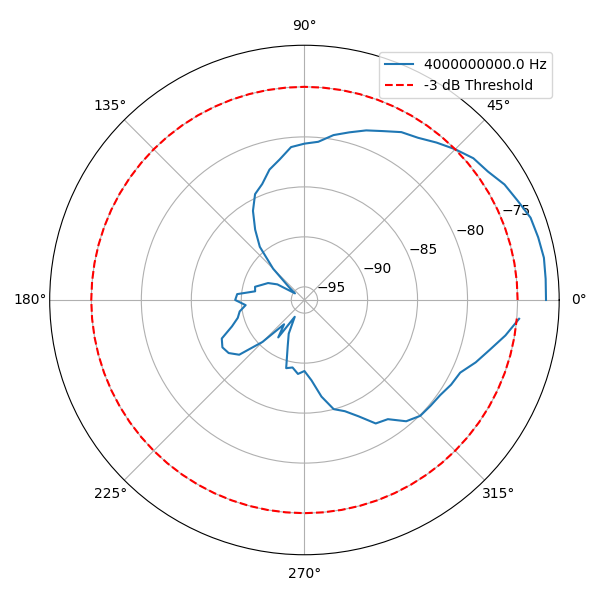
\includegraphics[width=0.8\linewidth]{./data/day5/polar_plot_4GHz.png}
    \caption{4GHzにおける放射パターン (極座標プロット)}
    \label{fig:polar_4GHz}
\end{figure}

\begin{figure}[h]
    \centering
    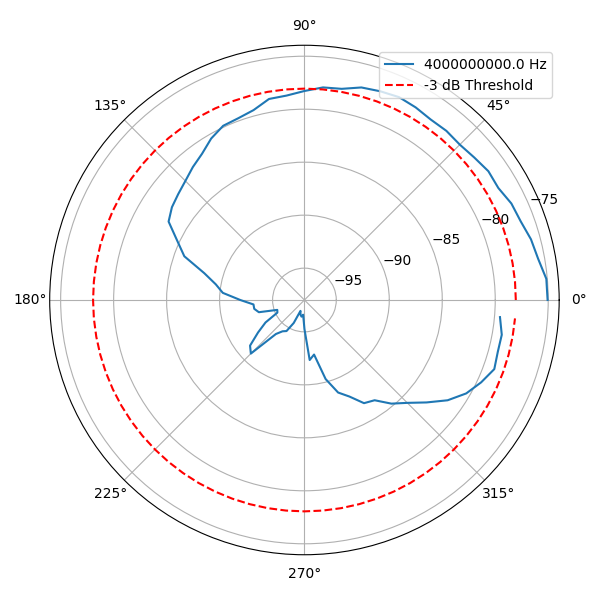
\includegraphics[width=0.8\linewidth]{./data/day5/polar_plot_8GHz.png}
    \caption{8GHzにおける放射パターン (極座標プロット)}
    \label{fig:polar_8GHz}
\end{figure}

\section{興味深い結果や事象について}
実験においては,シールド環境において計測を行った上,Wi-FiやBluetoothの周波数帯域である2.4 GHzや5 GHzの周波数帯域を避ける周波数を観測した.

実際,0度における放射強度を周波数ごとに観測をしたところ,2.4GHzや5GHzがほかの周波数に比べて大きいというようなことはなかった.


\subsection{参考文献}
文献は以下に示す.

\begin{thebibliography}{9}
  \bibitem{jemima}
  一般社団法人 日本電気計測器工業会,
  \textit{ネットワークアナライザ},
  \url{https://www.jemima.or.jp/tech/3-09-01.html},
  Accessed: 2024-12-07.

  \bibitem{ni}
  National Instruments,
  \textit{Introduction to Network Analyzer Measurements},
  \url{https://download.ni.com/evaluation/rf/Introduction_to_Network_Analyzer_Measurements.pdf},
  Accessed: 2024-12-07.

  \bibitem{coppermountain}
  Copper Mountain Technologies,
  \textit{How Does a Vector Network Analyzer Work?},
  \url{https://coppermountaintech.com/how-does-a-vector-network-analyzer-work/},
  Accessed: 2024-12-07.

  \bibitem{cqpub}
  CQ出版,
  \textit{マイクロストリップ線路でスタブを作る},
  \url{https://www.cqpub.co.jp/dwm/contents/0064/dwm006401270.pdf},
  Accessed: 2024-12-07.

  \begin{thebibliography}{9}
    \bibitem{highfreq-tutorial}
    High Frequency Electronics,
    \textit{A Tutorial on Antenna Basics},
    \url{https://www.highfrequencyelectronics.com/Mar09/HFE0309_Tutorial.pdf},
    Accessed: 2024-12-07.
\end{thebibliography}





\end{document}

